
%!subsection{Cultural Significance of Facades and Ornament}
%!\label{subsec: FacadeandOrnament}

%!==========================
%Delve deeper into how facades reflect cultural values, societal norms, and historical contexts. Explore how different societies and civilizations have expressed their identity through architectural ornamentation and symbolism.
%!==========================

%!Concise version
Architecture, transcending its primary role of providing shelter, serves as a canvas reflecting the cultural, historical, and societal narratives of its time.
Facades and ornamentation, in this context, become critical in conveying these narratives, bridging the gap between the aesthetic and the symbolic, and establishing the interface between buildings and their environments, influencing comfort and energy efficiency, while reflecting the building's identity\cite{Kamal2020}.

While the previous section traced the oscillations between simplicity and complexity in architectural styles to establish a foundation for the notion that contemporary architecture is gravitating towards a renaissance of complexity, here we explore the underlying cultural currents that influenced these shifts.
The evolution of facade design and ornamentation mirrors societal transformations, technological progress, and shifts in artistic sensibilities, each impacting how communities relate to their built environment.

%Facades according to Vitruvius

Vitruvius, in his 1st-century BCE work `De Architectura', outlined principles for architecture that emphasize structural soundness, functionality, and beauty\cite{Ostwald2023}.
He advocated for harmony and balance in design, using the principle of `Decor' to guide appropriate articulation that respects religious, natural, and social conventions\cite{Lefas2000}.
Vitruvius's principles, dormant for centuries, found renewed interest during the Renaissance and continued through the Neoclassical and Ecole des Beaux-Arts styles\cite{Wikipedia2023}.
This revival reinforced the classical architectural aesthetics rooted in order and rationality (Figure\ref{fig:Oldtimeline} c,e).
The principles of Vitruvius, emphasizing a balance of structural integrity, functionality, and aesthetics, have had a lasting impact, shaping the trajectory of architectural design and ornamentation throughout history.

%facade according to bernini and borromini

Moving beyond the Renaissance era and into the Baroque style, a significant shift in the perception of facades and ornamentation occurs.
Francesco Borromini, a prominent Italian architect of the Baroque period, emerges as a key figure in this context.
Borromini's architectural philosophy revolved around the facade as a reflection of a building's interior.
He viewed the facade not just as an ornamental feature but as a visual representation of the internal spaces and functions\cite{Benjamin2006}.
Borromini's designs often featured elaborate geometric patterns, curved forms, and sculptural elements, integrating the facade with the building's spatial organization and internal arrangement.
This approach is exemplified in his works, such as the San Carlo alle Quattro Fontane Church in Rome (Figure\ref{fig:Oldtimeline} d).

Borromini's perspective on facades transcended surface aesthetics.
He believed facades should express the building's deeper design and purpose, embodying an expressive display of interiority and an invitation for an external reading\cite{Biglieri2004}.
This philosophy underscores the integral role of facades in the overall architectural composition during the Baroque period.

% context on neo classic, art nouveau and art deco

In tracing the evolution of facades and ornamentation, it's important to recognize the architectural periods that significantly influenced the field, bridging the gap between the Baroque era and the transformative epoch of Modernism.
Notable styles in this transition include Neo-Classicism, Art Nouveau, and Art Deco.

Neo-Classical architecture (late 18th to early 19th centuries) revived Vitruvian principles and Palladian ideals.
It emphasized formal elegance and symmetry, often featuring facades with balanced proportions and columns (Figure\ref{fig:Oldtimeline} e).
Art Nouveau (late 19th to early 20th centuries), led by architects like Gaudi, introduced organic forms into facade design.
Gaudi's work, such as Casa Batlló, utilized flowing lines and natural motifs\cite{Nasir2022} (Figure\ref{fig:Middletimeline} a).
Art Deco (1920s to early 1930s) merged luxury and technological progress, characterized by geometric shapes, high-contrast colors, and metallic surfaces, as seen in the Chrysler Building\cite{Kotb2014} (Figure\ref{fig:Middletimeline} b).
While these styles contributed to the diversity of architectural aesthetics, they did not initiate the profound paradigm shifts that Modernism would later bring.
With this context, we now turn to the significant impact of the Modernist movement on architectural philosophy.

% Modernism and facade according to Le Corbusier

The transition into the 20th century's Modernist style marked a significant shift in the approach to facades and ornamentation.
As discussed in the previous section, this era, saw a move away from traditional ornamental design.

Loos, in his 1908 article `Ornament and Crime', a prominent figure on this movement, championed functional design and critiqued conventional ornamentation\cite{Saglam2014}.
Le Corbusier, a key Modernist architect, further revolutionized facade design.
His work, particularly `Towards a New Architecture'\cite{Studio2a2023} and `The Five Points of a New Architecture', emphasized minimalism and utility.
He advocated for facades that reflect a building's purpose and the well-being of its occupants, adhering to his human-centric design philosophy\cite{Virseda2021}.

Le Corbusier's concept of `Free design of the facade'\cite{Corbusier1986} allowed for innovative use of materials and structural elements to create functional ornamentation.
His designs often featured large windows, sunshades, and brise-soleil, prioritizing light, ventilation, and climate control while maintaining aesthetic integrity (Figure\ref{fig:Middletimeline} c).
Thus, Le Corbusier's views on facades represent a blend of clarity, rationality, and harmonious integration, rejecting excess adornment while celebrating structural innovation and technological advancements.

% Postmodernism and facade according to Venturi

Despite the innovative drive of Modernism, its utopian vision often fell short in materializing human-centric environments, leading to spaces that felt monotonous and detached from cultural contexts.
This paved the way for Robert Venturi's critical perspective on Modernism and his pioneering role in the Postmodernism movement.

Venturi, in his seminal works like `Complexity and Contradiction in Architecture' and `Learning From Las Vegas', challenged the Modernist ideals, advocating for architecture that embraced complexity, contradiction, and meaningful ornamentation \cite{Venturi1977}.
He criticized the Modernist approach for its oversimplification and lack of symbolic expression, arguing for an architecture that responds to cultural context and human experience (Figure\ref{fig:Middletimeline} d).

%!% Figures Methodology intro
    %% Methodology Flowchart
    \begin{figure*}[!htb]
        \centering
        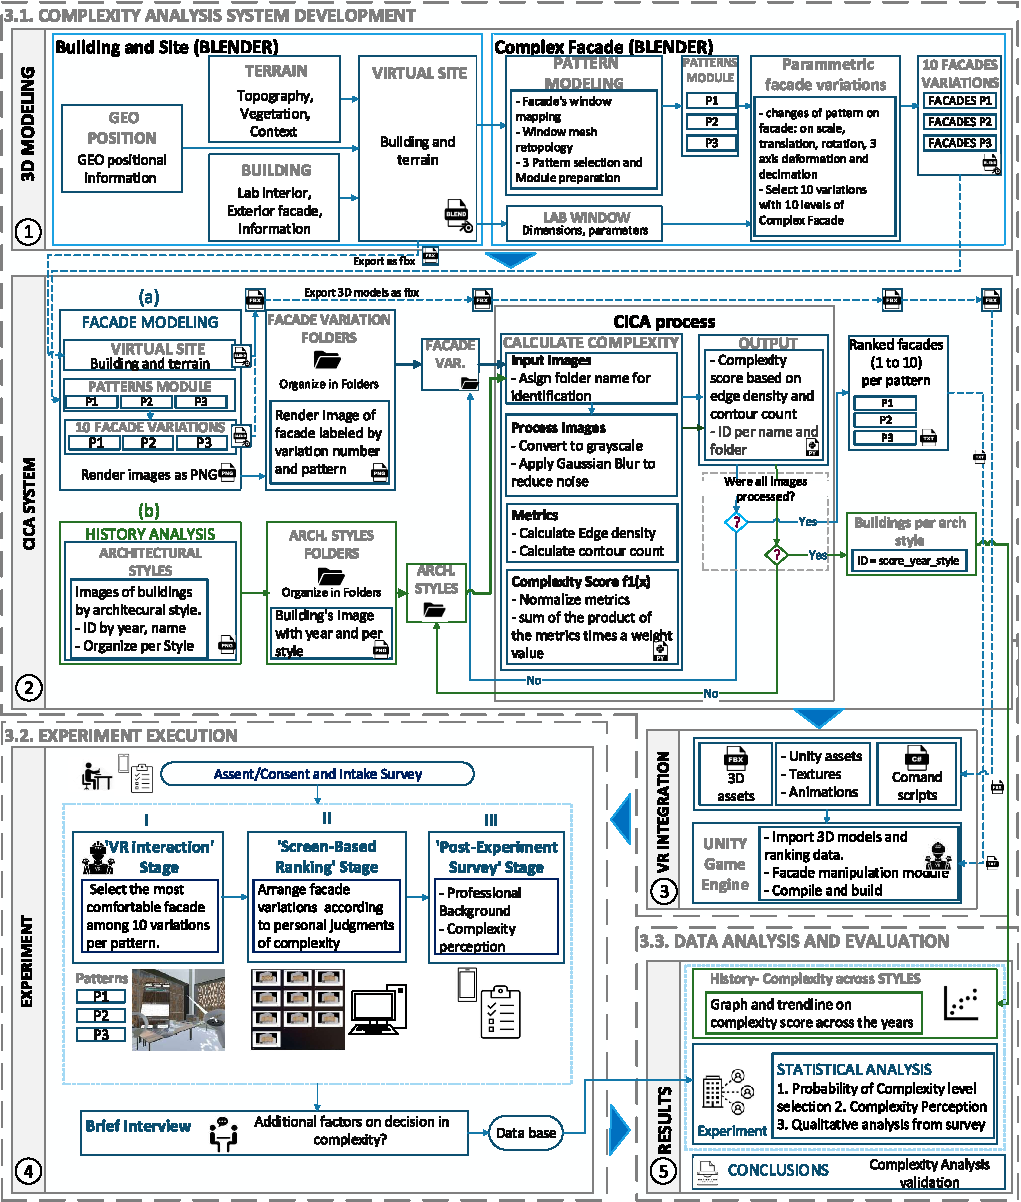
\includegraphics[width=\linewidth]{Images/MethodologyFlowchart}~\caption{Methodology Flowchart illustrating the sequential steps of this study's approach framework designed to assess the tolerance of users towards complex facade design. Higlighting the usage of the CICA system (as detailed in Section\ref{subsec:Computational Image Complexity analysis}) into the VR system development (detailed in Section\ref{subsec:VRsystemDevelopment}), and the transition to experiment design (described in Section\ref{subsec:Experiment_design}), culminating in post-experiment data analysis and results phase (presented in Section\ref{sec:Results}).}
          \label{fig:MethodologyFlowchart}
    \end{figure*}

Venturi's approach to facades and ornamentation incorporated diverse elements, historical references, and bright colors, challenging the minimalist ethos of Modernism.
He believed in the richness of symbolism and the importance of integrating elements from historical precedents into contemporary design\cite{Venturi1971}.
His famous dictum, `Less is a bore', encapsulated his critique of Modernist minimalism and his advocacy for thoughtful ornamentation.

Venturi's vision encouraged the use of facades as mediums to communicate various meanings, evoke emotions, and respond to their cultural and contextual surroundings.
His influence in Postmodernism expanded architectural horizons, urging architects to embrace diversity, historical resonance, and meaningful expression in their designs\cite{Lutolli2020, Stamp2016}

%Contemporary styles

Following Postmodernism, contemporary architecture witnessed a shift towards more dynamic and diverse styles, including Deconstructivism, Neofuturism, High-tech modernism, Parametricism, and Pragmatic utopianism.
These styles collectively signify a move towards complexity in facade design and ornamentation, influenced by advancements in technology and a focus on sustainability.

Deconstructivism, characterized by fragmentation and non-rectilinear shapes, was exemplified by architects like Frank Gehry, who integrated unconventional forms into their designs (Figure\ref{fig:contemporarytimeline} \textit{a}).
Neofuturism, represented by architects like Santiago Calatrava, embraced a futuristic aesthetic with dynamic, flowing forms (Figure\ref{fig:contemporarytimeline} \textit{b}).
High-tech modernism, or structural expressionism, focused on showcasing technological components and advanced materials, as seen in works by Renzo Piano and Norman Foster (Figure\ref{fig:contemporarytimeline} \textit{c}).
Parametricism, often associated with Zaha Hadid, utilized computational design to create intricate geometries and dynamic structures (Figure\ref{fig:contemporarytimeline} \textit{d}).
Pragmatic utopianism, exemplified by Bjarke Ingels, combined ambitious visions with practical solutions, focusing on functionality, sustainability, and meaningful ornamentation (Figure\ref{fig:contemporarytimeline} \textit{e}).
These styles reflect the architectural evolution from the late 20th century into the 21st, showcasing a variety of approaches to facades and ornamentation that blend tradition with innovation.


%conclusion
In conclusion, the journey through the evolution of facade and ornament theory reveals a rich tapestry of architectural ingenuity, shaped by cultural, technological, and artistic influences.
From the foundational principles of Vitruvius to the ornate expressions of the Baroque period, the functional minimalism of Modernism, and the eclectic approaches of Postmodernism, each era has contributed distinct perspectives on the relationship between a building's exterior and its intrinsic character.

Contemporary styles like Deconstructivism, Neofuturism, High-tech Modernism, Parametricism, and Pragmatic Utopianism (see Figure\ref{fig:contemporarytimeline}) further demonstrate the diversity and dynamism in current architectural practice.
These styles collectively underscore an ongoing dialogue between simplicity and complexity, tradition and innovation, functionality and aesthetics.

As we look towards the future, the continued evolution of facade and ornament theory will undoubtedly be influenced by emerging technologies, sustainability concerns, and the ever-changing needs of human societies, shaping the built environment in ways that are both imaginative and responsive to the world around us.

The cultural significance of facades extends beyond aesthetic appeal, contributing to a community's sense of identity and continuity.
As we look to the future, the challenge and opportunity lie in harnessing emerging technologies to create architecture that resonates with societal values and cultural diversity, thereby enriching the urban landscape.




